% stellar tracks plots
\begin{figure*}
  \centering
  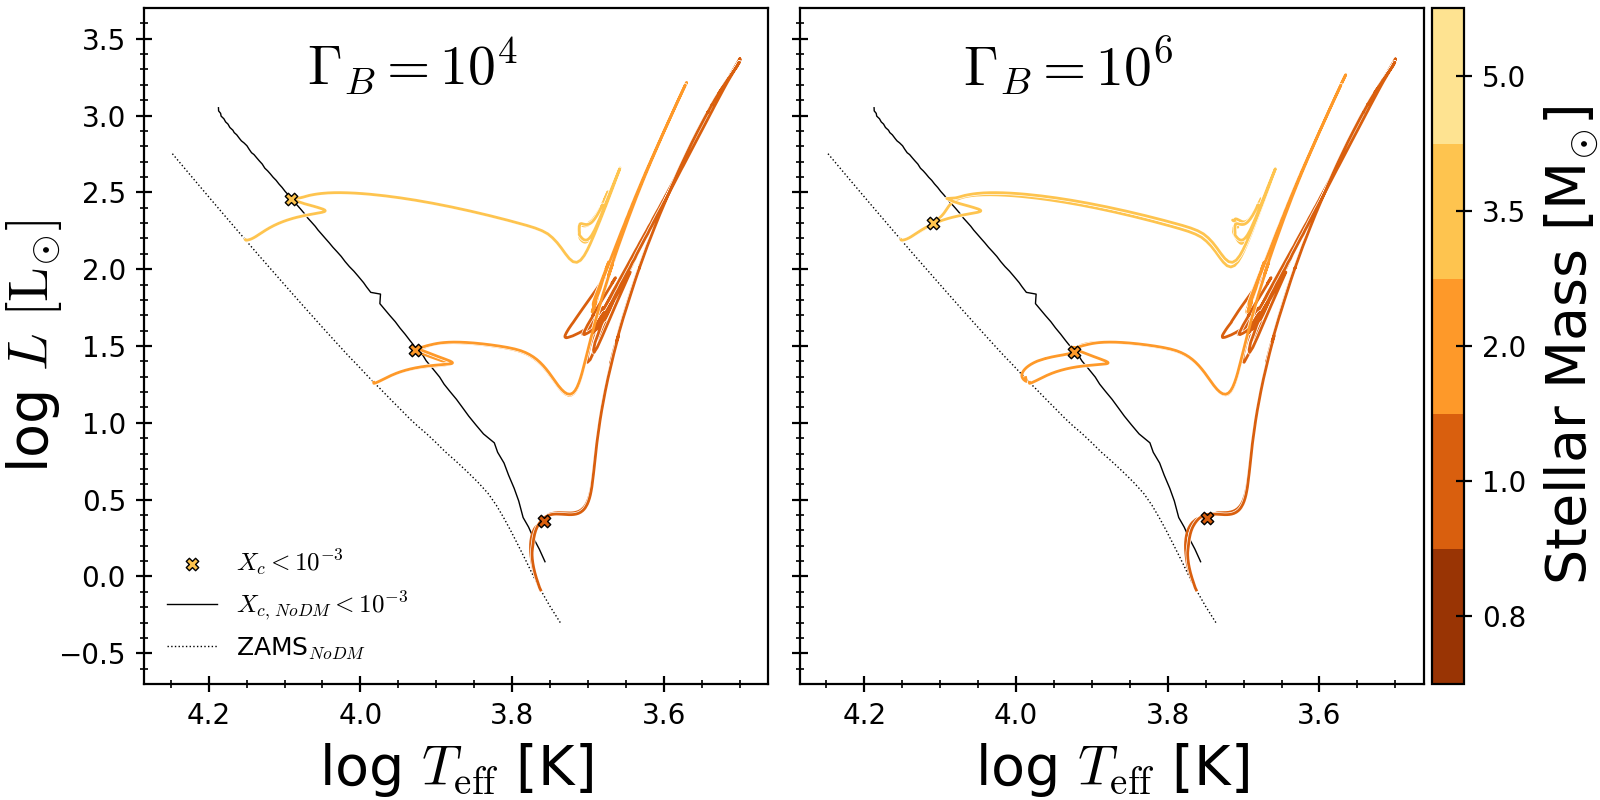
\includegraphics[width=\textwidth]{plots/tracks.png}
  \caption{
  Stellar evolution tracks from ZAMS to core helium depletion ($Y_c<10^{-12}$). x's mark the location where stars leave the MS, defined here as core hydrogen depletion below $X_c<10^{-3}$. For reference, the location of the ZAMS and core hydrogen depletion for \nodm models are plotted as dotted and solid black lines respectively.
  }
  \label{fig:tracks}

\end{figure*}


The effects of ADM on a single star's evolutionary track in an HR diagram (Fig.~\ref{fig:tracks}) are generally subtle since the most significant effect on the stellar surface properties $L$ and $\Teff$ is to move the star through roughly the same sequence of events at a more rapid pace. The location of the ZAMS is set by the balance between pressure support from nuclear burning and gravitational contraction, which depends only on the mass. The temperature of the red giant branch is set by an equilibrium between neutral and ionized hydrogen in the atmosphere. Hence, the star's HR track cannot be too different from the \nodm models.


% energy conservation and oscillations
Models with $\gb \gtrsim 10^4$ capture enough ADM so that $\epsx \gg \epspp$ near $r=0$ which destabilizes the core and sets up a series of oscillations.
As $\Tc$ continues to decrease, the temperature profile inverts and the center is no longer the hottest region in the star. Eventually, $\Tc < \Tx$ and dark matter begins moving energy back towards the center ($\epsx(r=0) > 0$, see Time 3 in Figure \ref{fig:m1p0_profs} \todo{possibly pick this time a little later, after xheat at center >0}). This increases both the central temperature and burning rate until $\Tc > \Tx$ and the cycle starts over. The effects propagate out to the surface where
$L$, $\Teff$, and $\Rstar$ all oscillate in response to changes in the core (Figure~\ref{fig:m1p0_kipp}). Similar oscillatory behavior was noted in \citet{Iocco2012} \qus{seems like I need to say more here, but I'm not sure what. The Iocco paper (arXiv:1201.5387v1) states the following: "In spite of our efforts, we have not been able to fully understand the reason of the oscillations seen in Figure 3, whether they are a physical effect arising from the “bouncing” of the central temperature on the WIMP temperature floor, or a numerical artifact. We have however checked that the existence of oscillations does not affect our results nor does change our conclusions. Beside the theoretical consistency of the intepretation presented in the paper, one can be convinced of the actual physical consistency of our results with observations based on several numerical experiments we have performed: ..."}.

The process repeats, with increasing amplitude, until the central temperature falls low enough that the core becomes significantly degenerate. Once electron degeneracy pressure can support the core, the temperature decouples from the equation of state and the star quickly settles into a more stable configuration with a significant temperature inversion (see Time 4 in Figures \ref{fig:m1p0_profs} and \ref{fig:m1p0_kipp}).

Overall, the ADM captured by these stars causes burning in a larger volume and at a higher rate than in standard models (see Figure \ref{fig:m1p0_kipp}). The stars then burn through the central hydrogen supply faster and leave the MS earlier: by 2.5 Gyr, solar mass stars with $\gbpow{6}$ have already left the MS and are climbing the red-giant branch. Note that the 2.5 Gyr, $\gbpow{6}$ isochrone is most similar the 10 Gyr, \nodm isochrone in Figure~\ref{fig:isos_cb}.
